\section{Backend Session Handling}

When a client is done loading all the application resources from the server, it 
will automatically open a WebSocket connection to the WebSocket server. This
WebSocket server is written on top of the Tornado web framework \cite{tornadoweb11}.
The initial WebSocket request contains the client's secret token to identify the
client and the user associated with this client. If the user has no session
already opened, a new ``WhalesSessionManager''\ref{fig:session management} is
created for this user. If the user already exists in a session manager, but on another client, the user is
added to the already existing session manager. In effect, this means that any
user can only be in one session, no matter how many places this user is logged
in to. This both enables the user to use one client simply as a ``remote'' to
control some other client that is hooked up to a stereo, but also prevents users
from sharing their account with other users. They would simply be placed in the
same session, and be forced to listen to whatever the other people on the same
account is listening to.

%TODO: without newline i got a bad box. It made me sad, but i cba to fix atm.
Inside the ``WhalesSessionManager'' instance, each user is stored in a\newline
``WhalesUserSession'' instance.


The ``WebSocketHandler'' acts as the connection
between client and server. When adding a new connection to a manager, the manager then runs through all connected users, checking if any other ``WhalesUserSession'' matches the new
user trying to connect. If a match is found, the new connection is linked to the 
already existing ``WhalesUserSession'' instance. If not, a new one is created
and added to the manager.


All incoming data from sessions in a manager is parsed along to the manager's
``WhalesPackageHandler'' object, that contains the different handlers. The
package handler holds a reference to the calling manager to be able to
comminicate with the clients connected to it. Below is listed the entry point
for every ``WhalesPackageHandler'' and the ``handle\_chat'' handler.

\begin{snippet}[language=Python,caption=Handler entry point]
def handle(self,package,connection):
	handler = getattr(WhalesPackageHandler,"handle_"+package['type'],WhalesPackageHandler.handle_default)
	if handler != None:
		handler(self,package,connection)
\end{snippet}

\begin{snippet}[language=Python,caption=The chat handler]
	def handle_chat(self,package,connection):
		for session in self.manager.sessions:
			session.write_message(encode(package))
\end{snippet}

%TODO: skal figuren ligge her, eller m�ske i starten af afsnittet?
\begin{figure}[!ht]
	\centering
		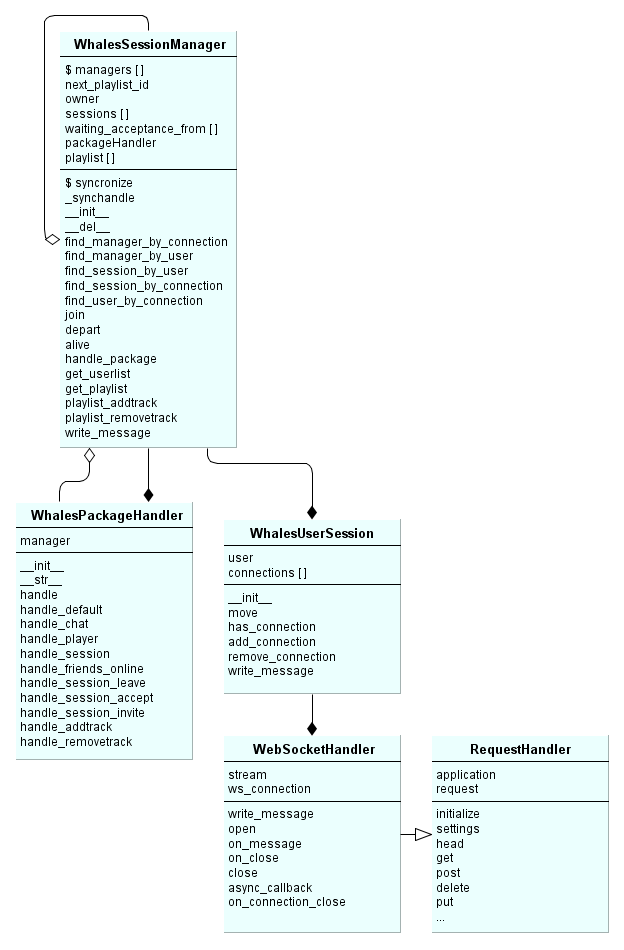
\includegraphics[width = 1.0\textwidth]{implementation/figures/session.png}
	\caption{Backend session management}
	\label{fig:session management}
\end{figure}
 
